%% V1.0
%% by Gabriel Garcia, gabrcg@gmail.com
%% This is a template for Udacity projects using IEEEtran.cls

%% Be Udacious!


\documentclass[10pt,journal,compsoc]{IEEEtran}

\usepackage[pdftex]{graphicx}    
\usepackage{cite}
\hyphenation{op-tical net-works semi-conduc-tor}

\newcommand{\subsubsubsection}[1]{\paragraph{#1}\mbox{}\\}

\setcounter{secnumdepth}{4}
\setcounter{tocdepth}{4}

\begin{document}

\title{Localization Project}



\author{Reinaldo Ossuna}

\markboth{Localization project, Robotics Nanodegree Program, Udacity}%
{}
\IEEEtitleabstractindextext{%

\begin{abstract}
  In this project we implemented the Monte Carlo algorigtm in two diferents robots created in a Gazebo/Rviz
  simulated environments, each equipped with laser range sensors and camera.Both robots successfully navigated in the
  provided map (Jackal Race car).
\end{abstract}

% Note that keywords are not normally used for peerreview papers.
\begin{IEEEkeywords}
Robot, Udacity, Localization, Monte Carlos, AMCL, Kalman Filter, EKF
\end{IEEEkeywords}}



\maketitle
\IEEEdisplaynontitleabstractindextext
\IEEEpeerreviewmaketitle
\section{Introduction}
\label{sec:introduction}

\IEEEPARstart{L}{ocalization} is the problem of the estimation of robot's pose relative to a map. Cox\cite{cox1991}
considers
localization the most fundamental problem to providing a mobile robot with autonomous capabilities.\\
There is many localization problems. The simplest one, is \textit{local localization}. Where the initial pose is known and the
principal task is to correct the errors in the robot's sensors. The \textit{global localization}, the robot's initial pose is
unknown and the robot has to determine it. We can cite more difficult problems, the \textit{kidnapped
robot} problem, in which the robot's pose can change any time. And the \textit{multi-robot localization} problem, where multiple robots
need to localize themselves.
\\In this project we'll focus on the global localization problem using ROS packages, this use a Augmented Monte Carlo
Localization algorithm, wich uses a partivle filter to track the pose of a robot against a know map.

\section{Background}

In this section we discuss the two principal approaches to the localization problem, Kalman filter and MCL.

\subsection{Kalman Filters}

The Kalman filter is a set of mathematics equations that is extensive used in area of autonomous or assisted
navigation.\\
The filter supports estimation of past, presents and even future states, and it can do so even when the precise nature
of the modeled system is unknown\cite{Welch1997}.

Unfortunately, Once into the nonlinear, non-Gaussian problems, most of the real system are nonlinear and no-Gausian, the
Kalman filter don't work very well. With this in mind was created the Extended Kalman filter, which on adapted
techniques from calculus, Taylor Series expansions, to linearize a model. 

\subsection{Particle Filters}

The Monte Carlo Localization (MCL) represent the belief by a set of weighted vector distributed in the global map. In
each period of time the vector are re-sampled and eventually converge to the robot's pose.


"MCL has been at the core of our robot navigation software. It's more efficient and accurate than any of our precious
algorithms" This citation from Sarkar prove the importance of MCL in the robotic field.\cite{Sarkar2009}.
\subsection{Comparison / Contrast}

MCL has many advantages over EKF, the Table~\ref{Tab:mclxekf} show a full comparison between the both algorithms, but 3
points can be exalted. MCL has a easier implementation, it's represent non-Gaussian distribution and it can approximate
any kind of distribution and the more important we can control the memory use.
\begin{table}[ht]
  \caption{MCL $\times$ EKF}
\begin{center}
  \begin{tabular}{l c c}
    \hline

    & MCL & EKF \\
    \hline
    Measurements & Raw Measurements & Landmarks\\
    Measurements Noise & Any & Gaussian \\
    Posterior & Particles & Gaussian \\
    Efficiency (memory) & A- & A+ \\
    Efficiency (time) & A- & A+ \\
    Ease of Implementation & A+ & A- \\
    Resolution & A- & A+\\
    Robustness & A+ & F \\
    Memory \& Resolution Control & Yes & No\\
    Global Localization & Yes & No \\

    State Space & Multimodel Discrete & Unimodal Continuous\\

    \hline
  \end{tabular}
  \label{Tab:mclxekf}
\end{center}
\end{table}

\section{Simulations}




This section should discuss the performance of robots in simulation. Items to include are the robot model design, packages used, and the parameters chosen for the robot to properly localize itself. The information provided here is critical if anyone would like to replicate your results. After all, the intent of reports such as these are to convey information and build upon ideas so you want to ensure others can validate your process.
You should have at least two images here: one that shows your standard robot used in the first part of the project, and a second robot that you modified / built that is different from the first robot. Remember to watermark all of your images as well. 

\subsection{Achievements}

Both robots reached the end goal in the map. Beside that more 4 goals was added to the navigation stack and both robots
reached all goals.

% Robot Models
\subsection{Benchmark Model}
\subsubsection{Model design}

The provided robot has a rectangular prism chassis with a size of 0.4, 0.2, 0.1. It's has two casters in spherical
shape with radius of 0.05 and two wheels with radius of 0.1.

\subsubsection{Packages Used}

\begin{itemize}
  \item AMCL\\
    A probabilistic localization system for a robot moving in 2D. it implements the Adaptive Monte Carlo Localization
    (AMCL), which uses a particle filter to track the pose of a robot against a known map.
  \item Navigation Stack\\
    A 2D navigation stack thtat takes in information from odometry, sensor streams, and a goal pose and outputs safe
    velocity commands that are sent to a mobile base.
  \item Turtlebot Teleop\\
    Provides teleoperation using keyboard
  \item Drive bot\\
    Define 5 goals to the Navigation Stack

\end{itemize}


\begin{figure}[thpb]
      \centering
      \includegraphics[width=\linewidth]{rosgraph.png}
      \caption{RQT graph}
      \label{fig:rqt}
\end{figure}

\subsubsection{Parameters}

\subsubsubsection{AMCL}\par
    All parameter below are necessary to increase the performace of the algorithms. This parametes can be higher depending on
    the hardware.
    The quantity of particles is quite low, but with a small number of particles they converge much faster and much
    preciser.
\begin{itemize}
  \item transform\_tolerance\\ 
        Time with which to post-date the transform that is published, to indicate that this is valid into the future \\
        value= 0.3

   \item min\_particles\\
        Minumum allowed number of particles.\\
        value= 5

   \item max\_particles \\
        Maximum allowed number of particles\\
        value= 25

    \item controller\_frequency\\
      The frequency at which this controller will be called in Hz\\
      value= 12
\end{itemize}

\subsubsubsection{Costmap Parameters}
\begin{itemize}
  \item obstacle\_range\\
    The default maximum distance from the robot at which an obstacle will be inserted into the cost map in meters.\\
    Value= 2.5\\

  \item raytrace\_range\\
    This parameter is used to clear and update the free space in the costmap as the robot moves\\
    Value= 3.0  \\
  \item inflation\_radius\\
    This parameter determines the minumum distance between the robot geometry and the obstacles. See
    Fig:\ref{fig:inflation}\\
    Value= 0.55
  \item width and height\\
    The width and height of the map in meters.\\
    Global= 10,10\\
    Local= 5.0,5.0
 \item resolution\\
   The resolution of the map in meteres/cell.\\
    Global= 0.05\\
    Local= 0.02
  \item rolling\_windows\\
    Whether or not to use a roling window version of the costmap\\
    Glogal= False\\
    Local= True
  \item pdist\_scale\\
    The weighting for how much the controller should stay close to the path it was given.\\
    Value= 0.6
  \item gdist\_scale\\
    The weighting for how much the controller should attempt to reach it local goal, also controls speed.\\
    Value= 0.8


\end{itemize}

\begin{figure}[thpb]
      \centering
      \includegraphics[width=\linewidth]{costmap-with-without-inflation.png}
      \caption{Low $\times$ High inflation radius}
      \label{fig:inflation}
\end{figure}


\subsection{MeineBot Model}
% ditto
\subsubsection{Model design}

This model has design based in a real robot, Fig:\ref{fig:model}. All the robot was created using macros and
constants values to easy resize the robot if necessary.\\
The robot is a rectacle with size of 0.1, 0.2 with just one caster and a battery and the rasbery pi in the back used to
counterbalance. Like the Udacitybot, it has one camera and a ranger finder.

\begin{figure}[thpb]
      \centering
      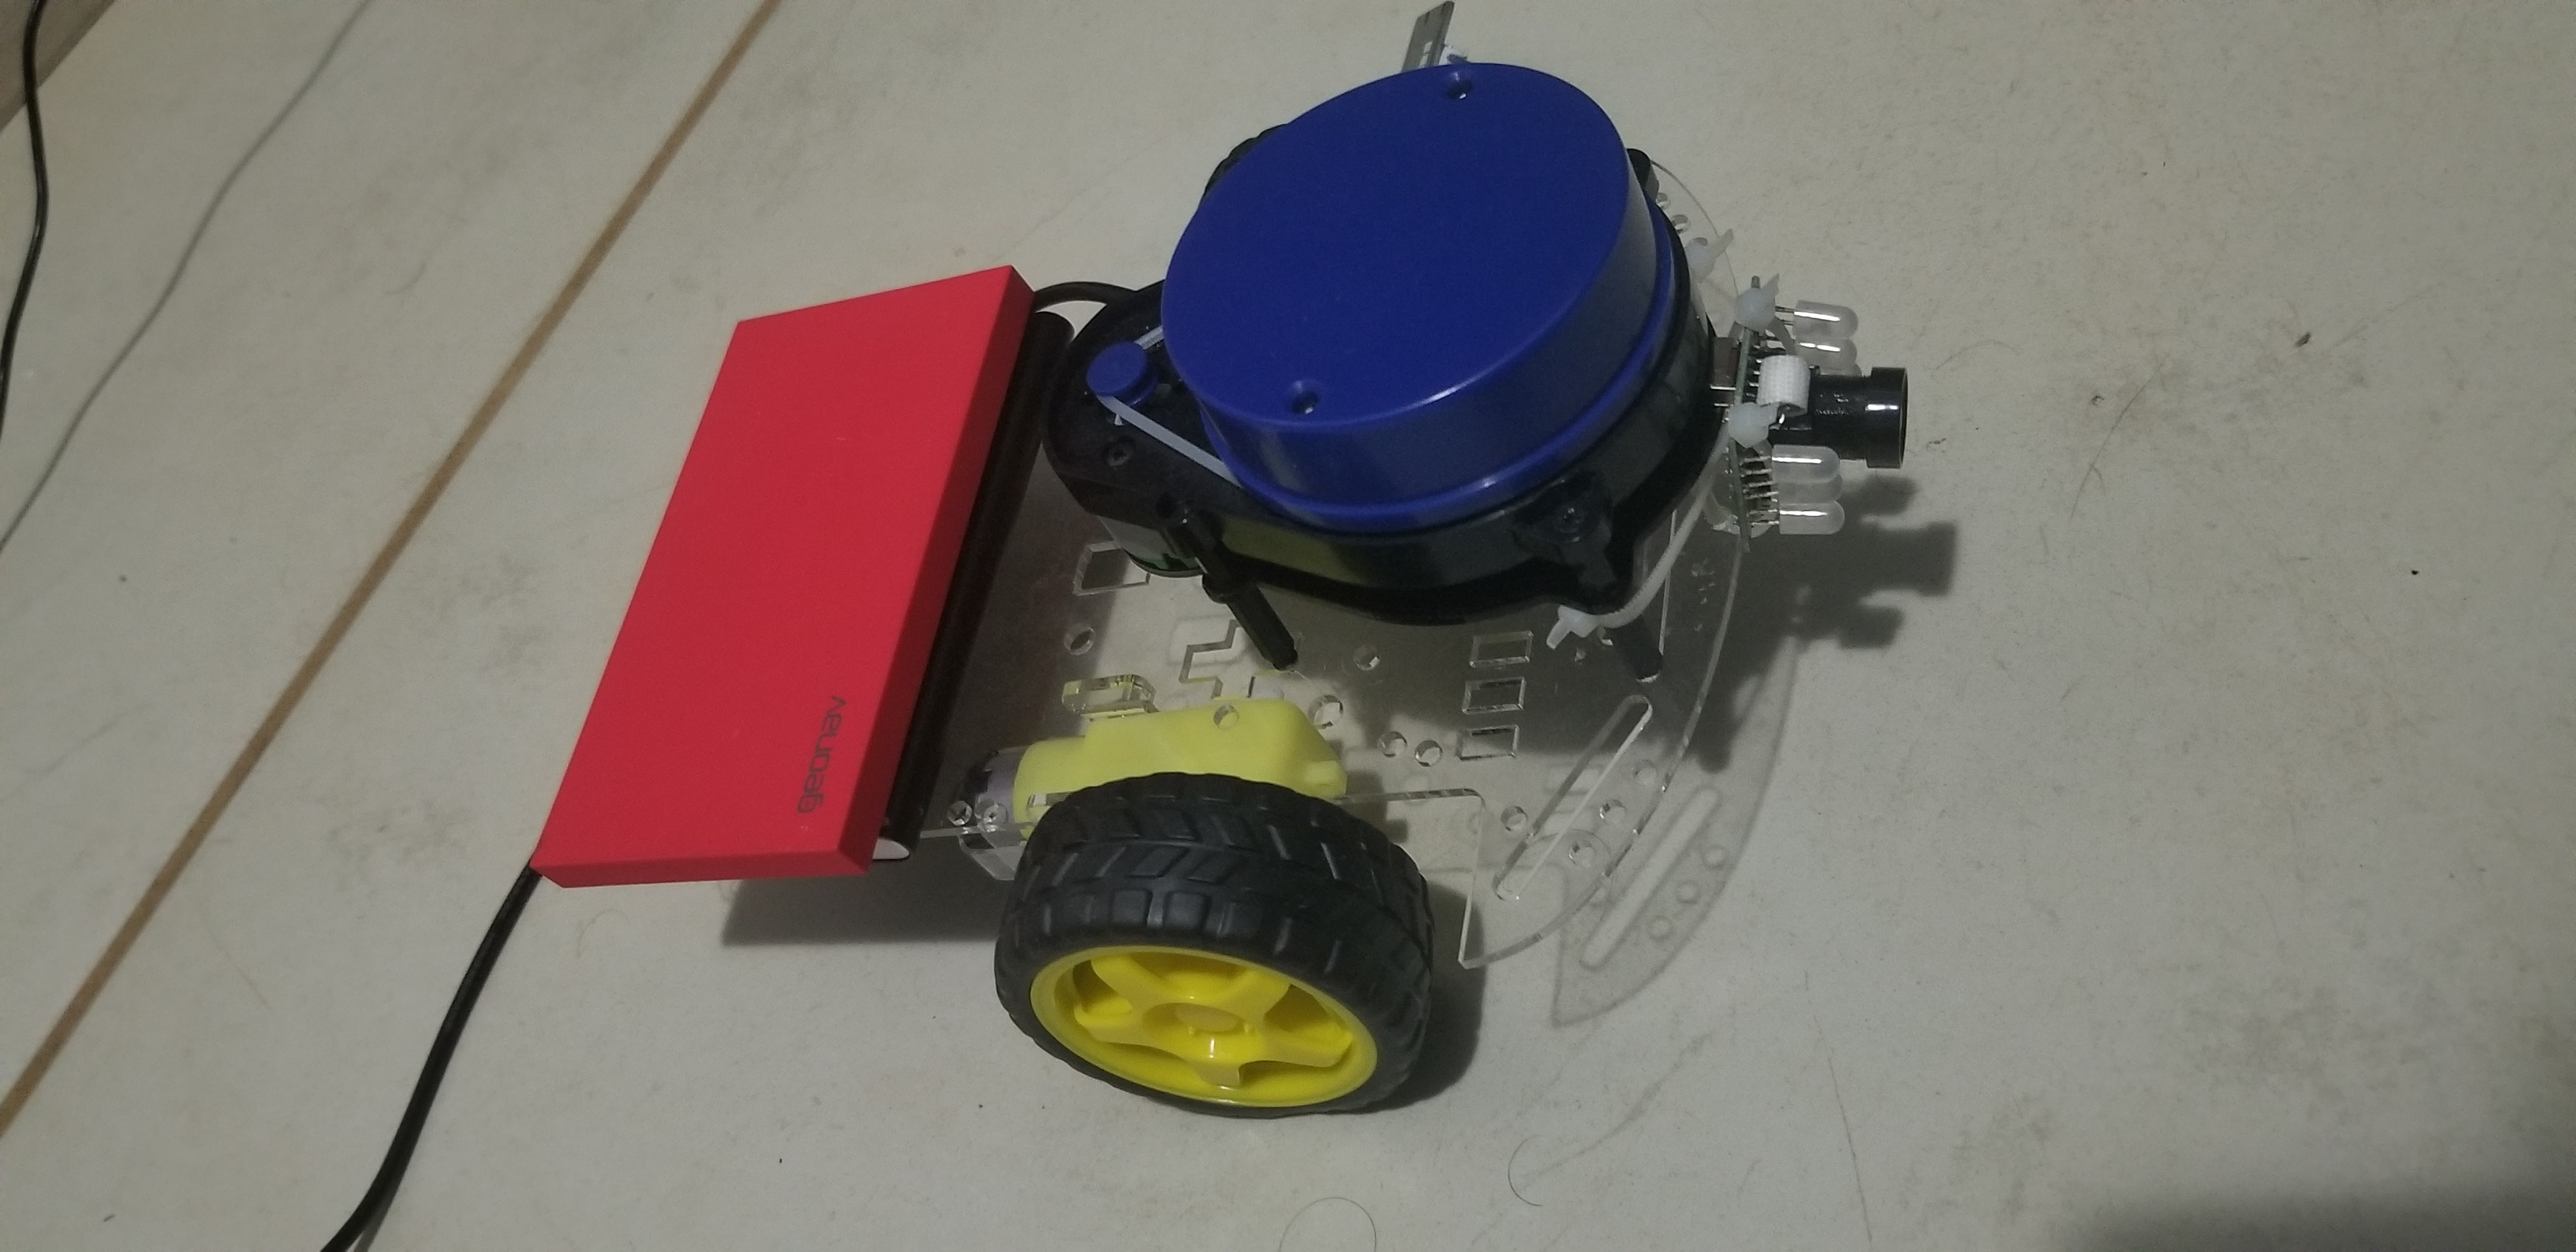
\includegraphics[width=\linewidth]{model.jpg}
      \caption{Real Model}
      \label{fig:model}
\end{figure}

\subsubsection{Packages Used}
The same packages used in the Udacity bot
\subsubsection{Parameters}

Almost all values used in the udacity bot were reused in MeineBot.\\
\begin{itemize}
  \item inflatius\_radius\\
    Size my robot is quite small, the controler tried to pass between the barrel and the wall.
    Value= 0.9
   \item controller\_frequency
     The MeineBot is much faster that the udacityBot and the terminal start to print missed controller.\\
     value= 10
\end{itemize}


\section{Results}

Both models navigated very well, size MeineBot is smaller, it was much faster and this could bring some problems in the
navigation stack. 

\begin{figure}[thpb]
      \centering
      \includegraphics[width=\linewidth]{udacity-bot.png}
      \caption{Udacity bot Goal}
      \label{fig:udacitybot}
\end{figure}

\begin{figure}[thpb]
      \centering
      \includegraphics[width=\linewidth]{meine_bot_checkpoint.png}
      \caption{Meinebot Goal}
      \label{fig:meinebot}
\end{figure}



\subsection{Localization Results}
\subsubsection{Benchmark}
\subsubsection{Student}

\subsection{Technical Comparison} % only facts

The MeineBot has a bigger problem, size it's has just one caster and depends the of counterbalance from the baterry.
    This could induce some type of accident.
    Another aspect to observe is the ranger finder from the MeineBot is not parallel to the ground.
\section{Discussion}

\begin{itemize}
\item Which robot performed better?\\
  In the localization aspect both robots worked very well. In the velocity aspect MeineBot performed much better.
\item How would you approach the 'Kidnapped Robot' problem?\\
  The AMCL can solve the 'Kidnapped robot problem', size it's add random particles in each re-sampling.
\item What types of scenario could localization be performed?\\
  In know and closed places, without people walking around.
  
\item Where would you use MCL/AMCL in an industry domain?\\
  The MCL/AMCL would work very well in warehouse or any industry domain.
\item Localization accuracy and processing time.


  The trade between accuracy and processing depends on the number of particles used. With a increase of the number of
    particles the processing time increase but a good accuracy can be archivied with a small number of particles, this
    was showed in this project.

\end{itemize}

\section{Conclusion / Future work}

The AMCL is a powerful tool in the robotic. The fact the all of the algorith is ready to use as a ROS package is
    facinating. With small adjust in parameter we are able to deploy this powerful tool.\\
    In the future, deploy the model in a real world and perfome similar task performed here. And the use of SLAM
    algorithm to map a unknown enviroment. 


\nocite{*}
\bibliography{bib}
\bibliographystyle{ieeetr}

\end{document}
